\chapter{Episode-wise reward dynamics}
\label{chap:reward_structure}
\begin{quotation}
\noindent ``\emph{The Panic Monster is dormant most of the time, but he 
	suddenly wakes up when a deadline gets too close or when there's danger
	of public embarrassment, a career disaster, or some other scary 
	consequence.}''
\begin{flushright}\textbf{Tim Urban}, on procrastination\end{flushright}
\end{quotation}

Let us now look at why the reward of the first episode in a dual-episode
trial drops to random policy level when we know the agent is able to receive
an almost perfect reward in a single-episode trial. To understand why, we will
keep the same setting as previously, but
we will vary the length (in number of episodes) of the trials and the
discount factor $\gamma$.

\section{Inherent laziness}
There is a recurrent pattern visible in Figure~\ref{fig:20permsLR_training}.
Indeed, no matter the number of episodes in each trial, the last one will
always reach optimal or near-optimal performance while all previous episodes
will receive a reward which corresponds to following a random policy.\\

This is confirmed by the plots of Figure~\ref{fig:20permsLR_rewards} which
show the rewards obtained by playing several trials of 2 and 5 episodes
(after having trained on trials of corresponding length) over all the
permutations of the training set. Only the last episode of the trial will
succeed or almost succeed.\\

We will explain why the reward structure of the CartPole problem (+1 at
every time step) inevitably produces such an undesired behaviour and look
for ways to counter it.
\begin{figure}
	\centering
	\subfloat[][Training over 1 episode]{
		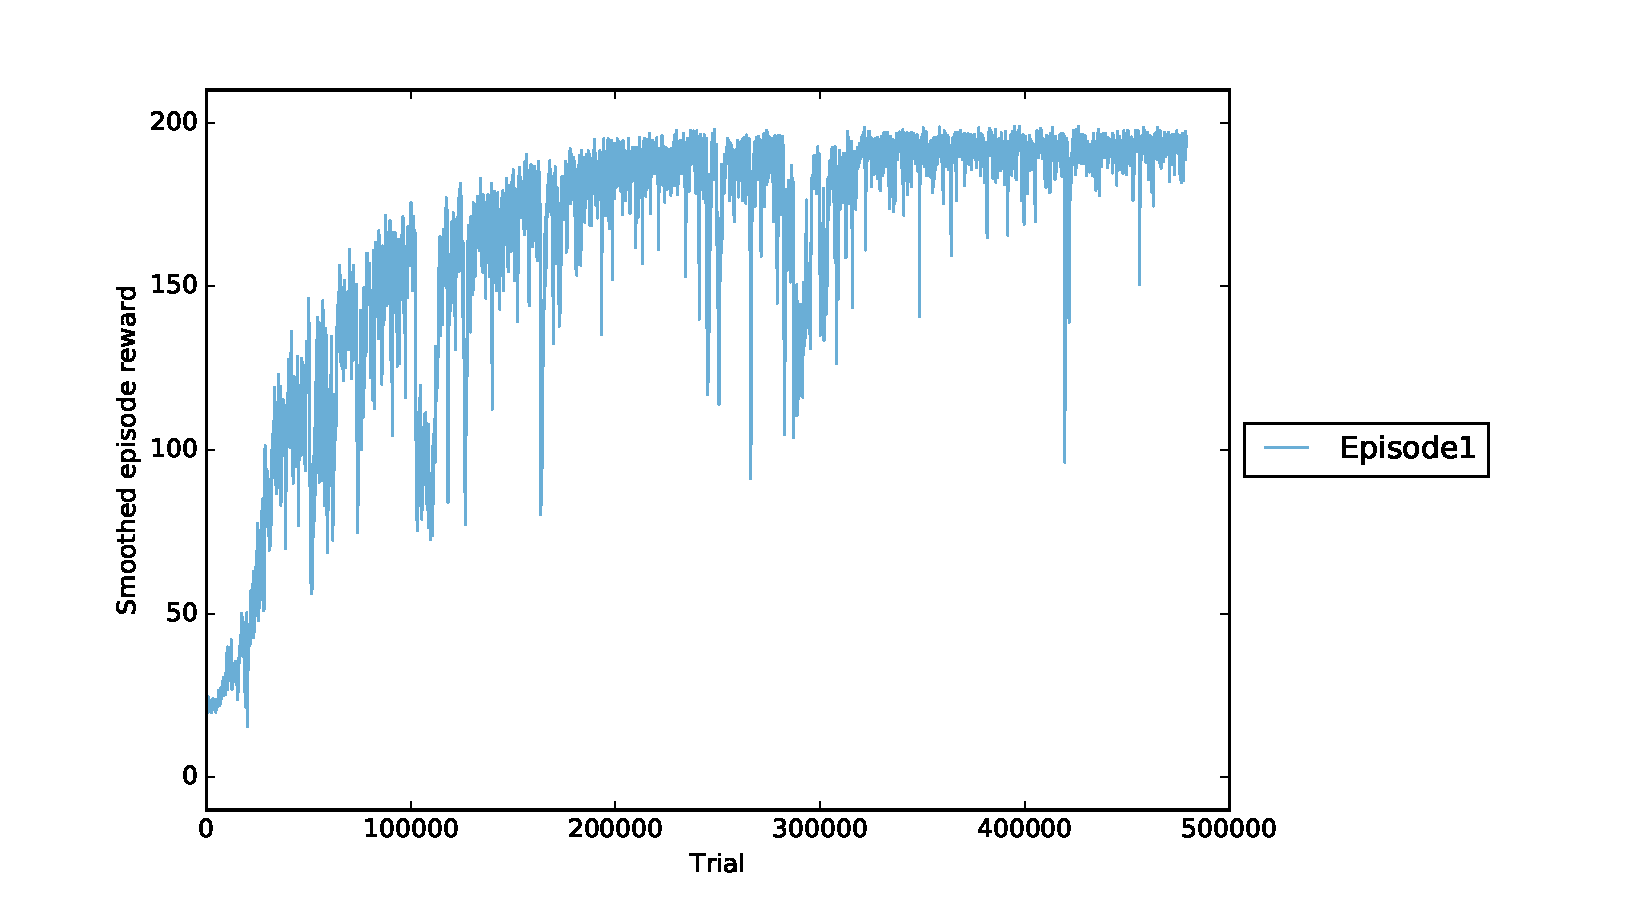
\includegraphics[width=0.49\linewidth]{fig/20permsLR1ep_training.pdf}}
	\subfloat[][Training over 2 episodes]{
		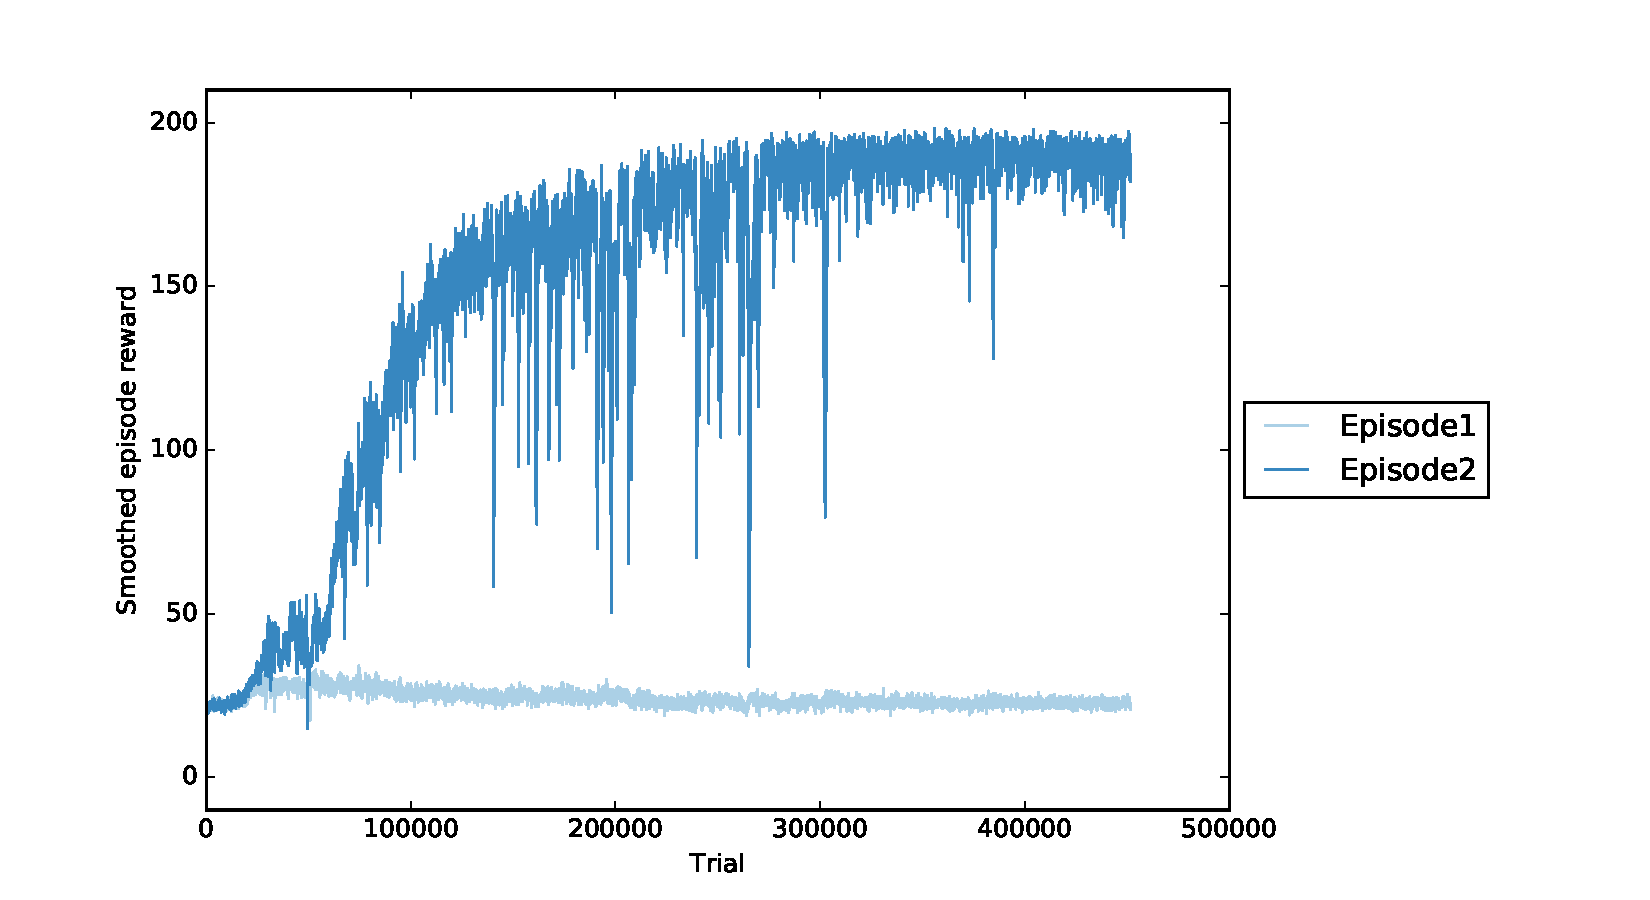
\includegraphics[width=0.49\linewidth]{fig/20permsLR2ep_training.pdf}}
	\\
	\subfloat[][Training over 5 episodes]{
		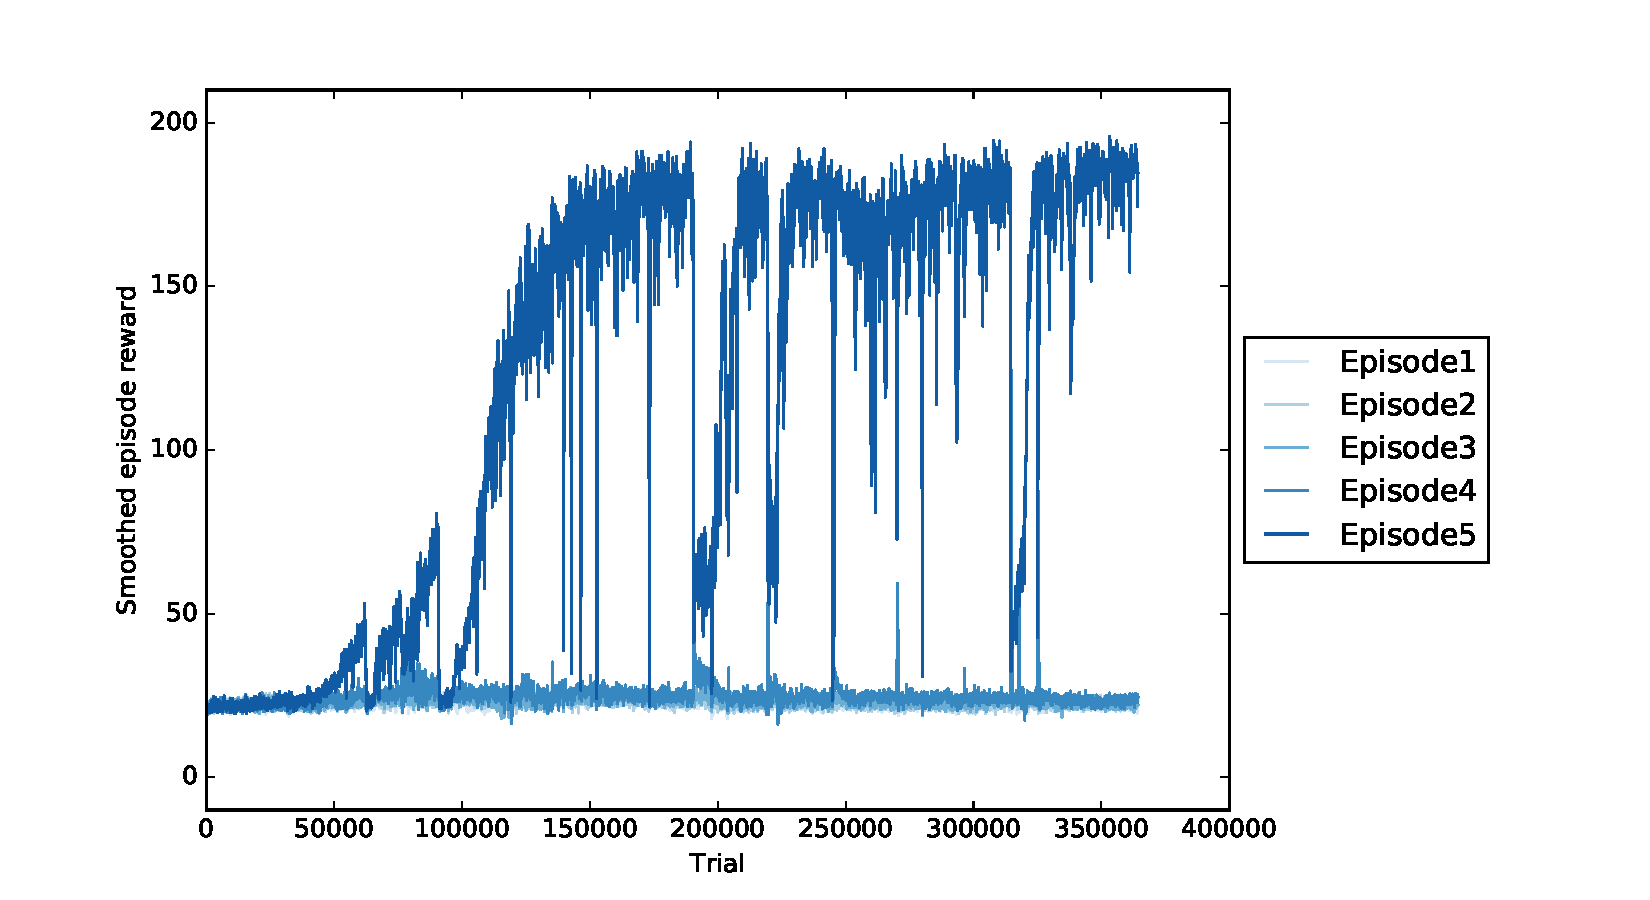
\includegraphics[width=0.9\linewidth]{fig/20permsLR5ep_training.pdf}}
	\caption{Episode-wise reward evolution when training on trials of 
	different lenghts}
	\label{fig:20permsLR_training}
\end{figure}

\begin{figure}
	\centering
	\subfloat[][2 episodes]{
		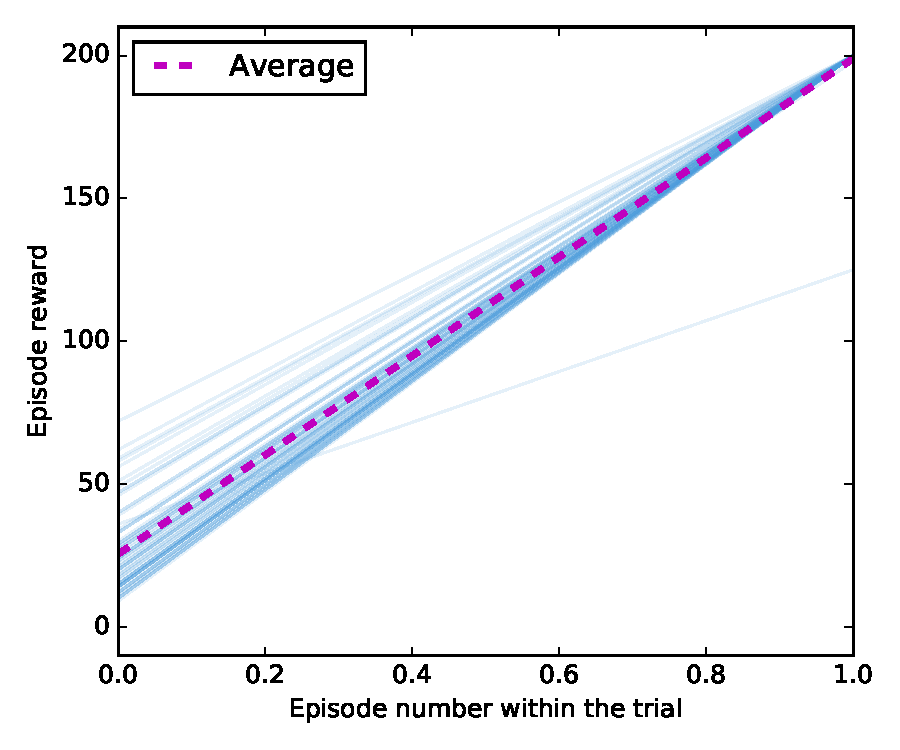
\includegraphics[width=0.4\linewidth]{fig/20permsLR2ep_rewards.pdf}}
	\subfloat[][5 episodes]{
		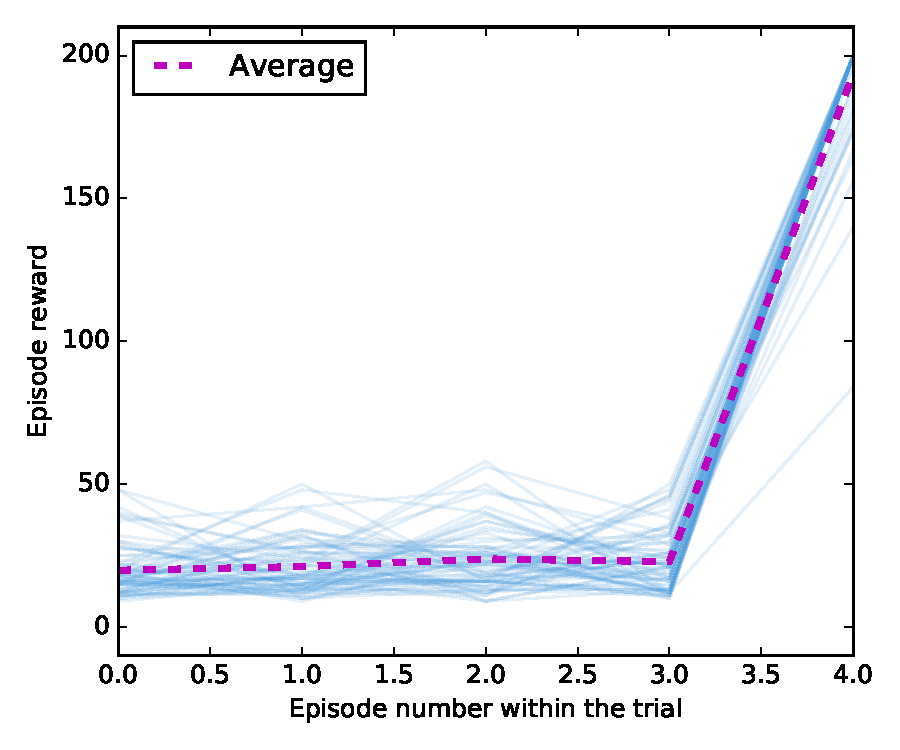
\includegraphics[width=0.4\linewidth]{fig/20permsLR5ep_rewards.pdf}}
	\caption{Testing performance of agents trained on trials of different
	lenghts. Several runs are displayed in blue on the same plot, and their
	average is shown as a red dashed line.}
	\label{fig:20permsLR_rewards}
\end{figure}

\begin{figure}
	\centering
	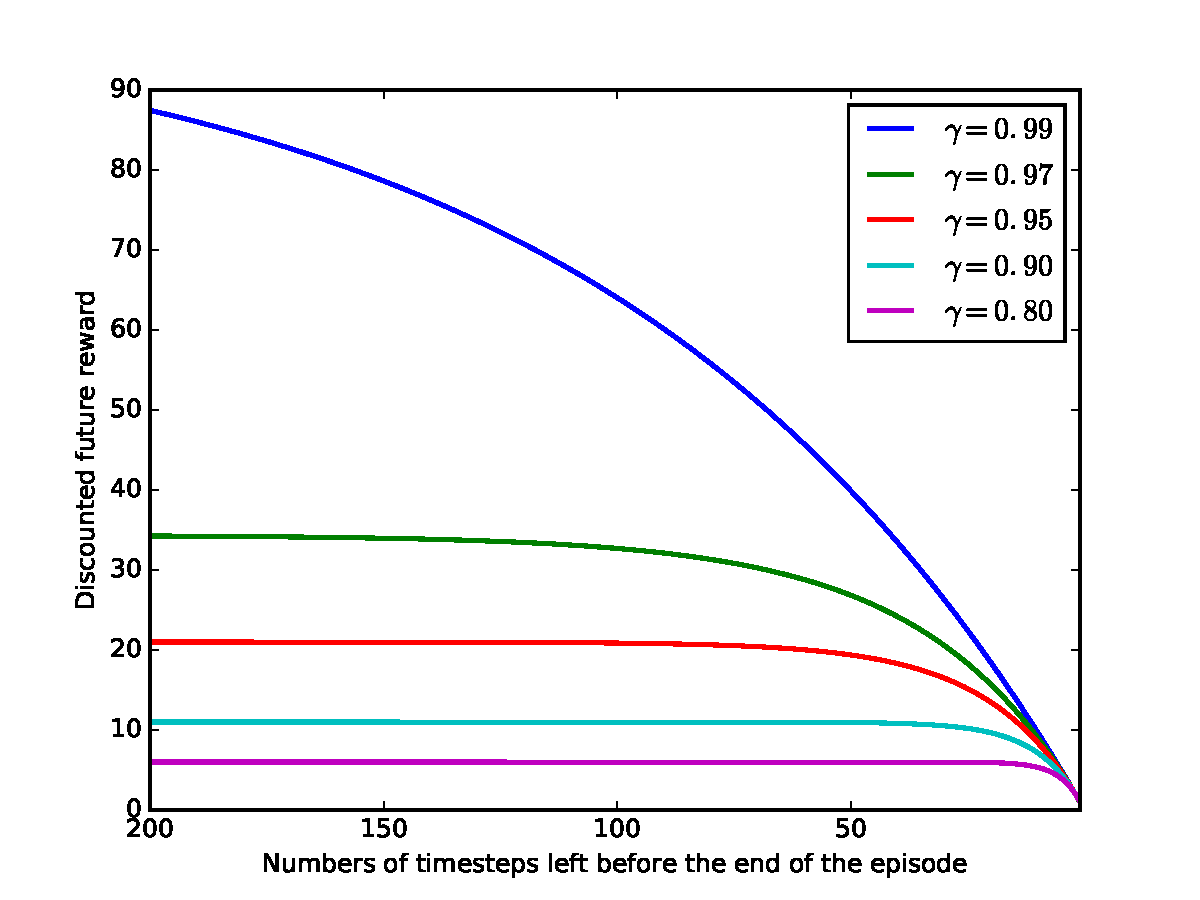
\includegraphics[width=0.8\linewidth]{fig/gamma_impact.pdf}
	\caption{Value of the discounted expected reward $R_t$ as a function
	of the number of timesteps left before the end of an episode in which
	a reward of +1 is given at every timestep; shown for different values
	of $\gamma$.}
	\label{fig:gamma_impact}
\end{figure}

\subsection{Problems with a 1-per-timestep reward}
\label{section:problems_1_timestep_reward}
This behaviour is linked to the dynamics of the expected future reward, 
the chosen discount factor and the reward structure of the environment.
In our case, the environment gives a constant +1 reward at every timestep of
a CartPole episode. If we choose a discount factor $\gamma=0.9$, the
discounted future reward at timesteps which are more than 50 timesteps away
from the end of the episode will be almost exactly equal (see 
Figure~\ref{fig:gamma_impact}).\\

This means that if an action that defines whether the episode ends or continues
at time $t$ has to be taken before time $t-50$, there is no way to link the
end of the episode with the action that was wrongly taken. This can be turned
around to say that actions do not really matter as long as the end of the
constant reward stream is more than 50 timesteps away for $\gamma=0.9$. In
our case, this explains why all episodes prior to the last one achieve low
reward. Because in every case, if the last episode is longer than 50
timesteps, the end of the reward stream is too far for the second-to-last 
episode to take it into account (if $\gamma=0.9$).\\

This should make the reader wonder why the last episode lasts more for more
than 50 ticks. As stated above, in episodes that are not the last one, a
failure doesn't lead to a loss in expected reward; at the contrary, the reward
stream keeps going after the end of the episode. For the last episode however,
the agent might notice that the current state of the environment will lead
to the end of the episode \textbf{and} of the trial, so the end of the 
reward stream if it doesn't take any action.\\

This reasoning assumes that the agent knows when it is playing the last episode;
and the results show that, in some way or another, the agent has learned to
count either the termination flags, or the number of timesteps needed
to get to the last episode. This will be analysed further in section 
\ref{section:beyond:moreeps}.

\section{Encouraging the agent to succeed}
There are two main parameters that directly affect this lazy behaviour : the
number of episodes in a trial and the discount factor. In the following
experiments, we will select a small subset of the training set previously 
used to accelerate training. This subset is shown in table~\ref{tab:3perms}.

\begin{table}
	\centering
	\caption{State permutations used for training and testing}
	\label{tab:3perms}
	\subfloat[Training distribution]{
		\bgroup
		\def\arraystretch{1.5}
		\begin{tabular}{c|c|c}
			[0, 1, 2, 3] & [0, 1, 3, 2] & [1, 0, 2, 3]
		\end{tabular}
		\egroup
	}
	\subfloat[Testing distribution]{
		\quad\quad
		\bgroup
		\def\arraystretch{1.5}
		\begin{tabular}{c}
			[1, 0, 3, 2]
		\end{tabular}
		\egroup
		\quad\quad
	}
\end{table}

\subsection{Tuning the discount factor}
If we want to enforce good performance for non-terminal episodes, selecting
higher values for the discount factor is the first solution that comes to mind.
Unfortunately, besides the fact that this only enforces $k$ last episodes
to have a high reward (instead of trying to maximise performance as soon as
possible), this solution doesn't seem to work, as Figure~\ref{fig:varied_gamma}
shows.\\

In this experiment, we selected 3 training permutations (see 
Table~\ref{tab:3perms}) and trained our agent for 5 episodes. Several trainings
were run with different values for the discount factor $\gamma$.\\

Even though the rewards of previous episodes clearly climb higher as
we increase the discount factor, they all eventually decline to random
policy-like reward. Once the discount factor reaches values where the
second-to-last episode should be involved in having a high reward (around
0.97 and above), training diverges and the agent never manages to reach
high scores.

\begin{figure}
	\centering
	\subfloat[][$\gamma=0.82$]{
		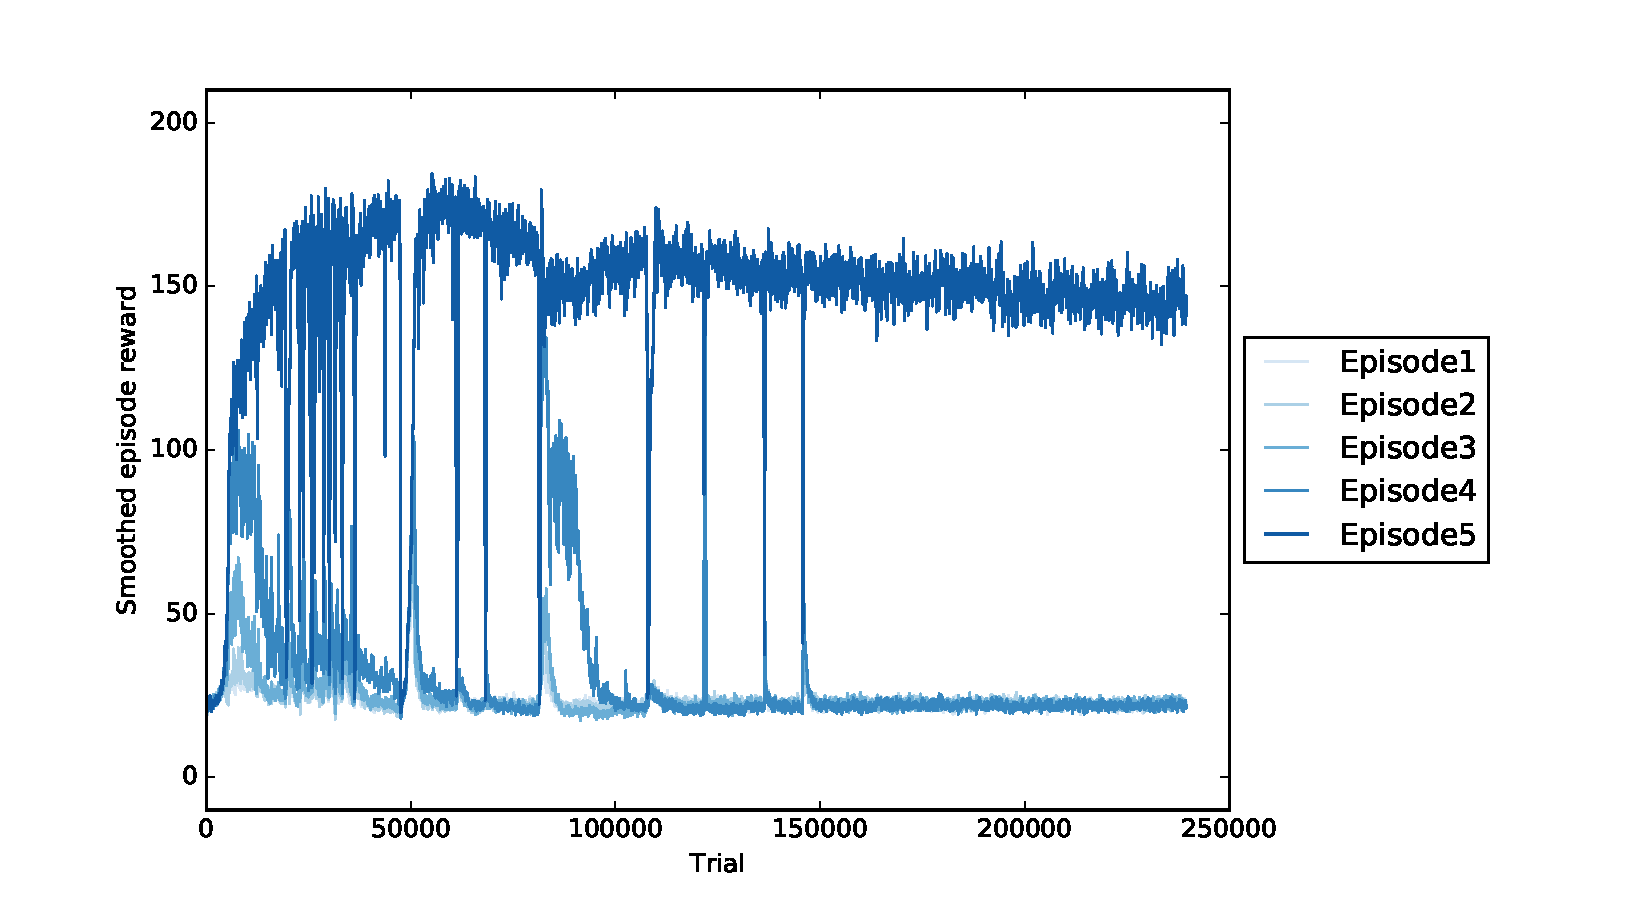
\includegraphics[width=0.49\linewidth]{fig/res_perms5ep_82.pdf}}
	\subfloat[][$\gamma=0.85$]{
		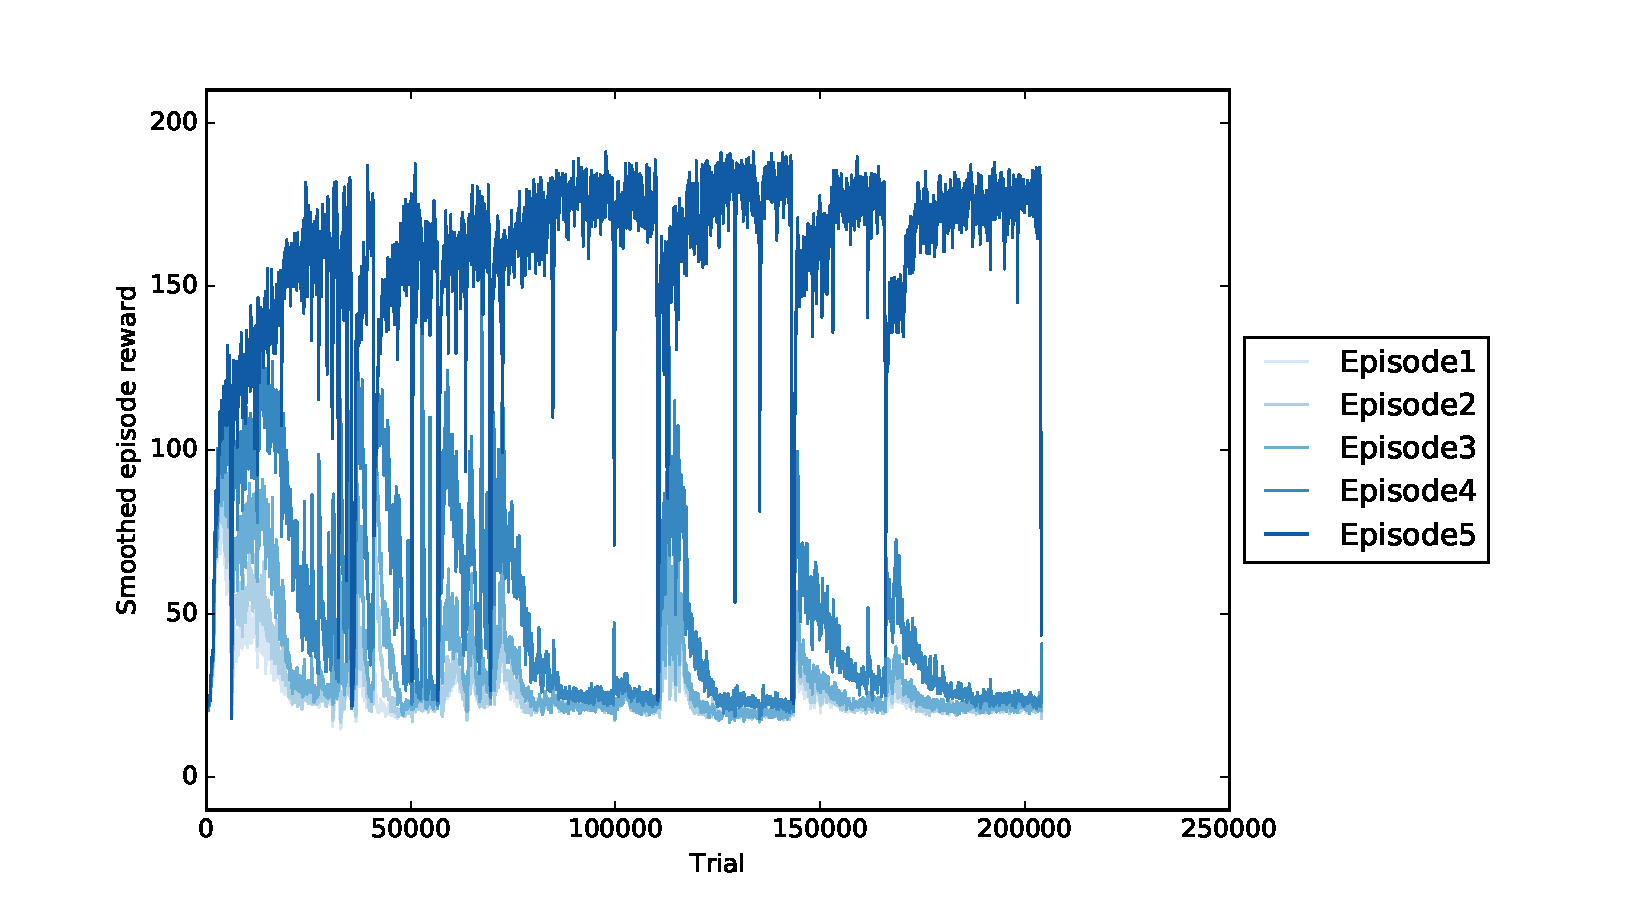
\includegraphics[width=0.49\linewidth]{fig/res_perms5ep_85.pdf}}
	\\
	\subfloat[][$\gamma=0.88$]{
		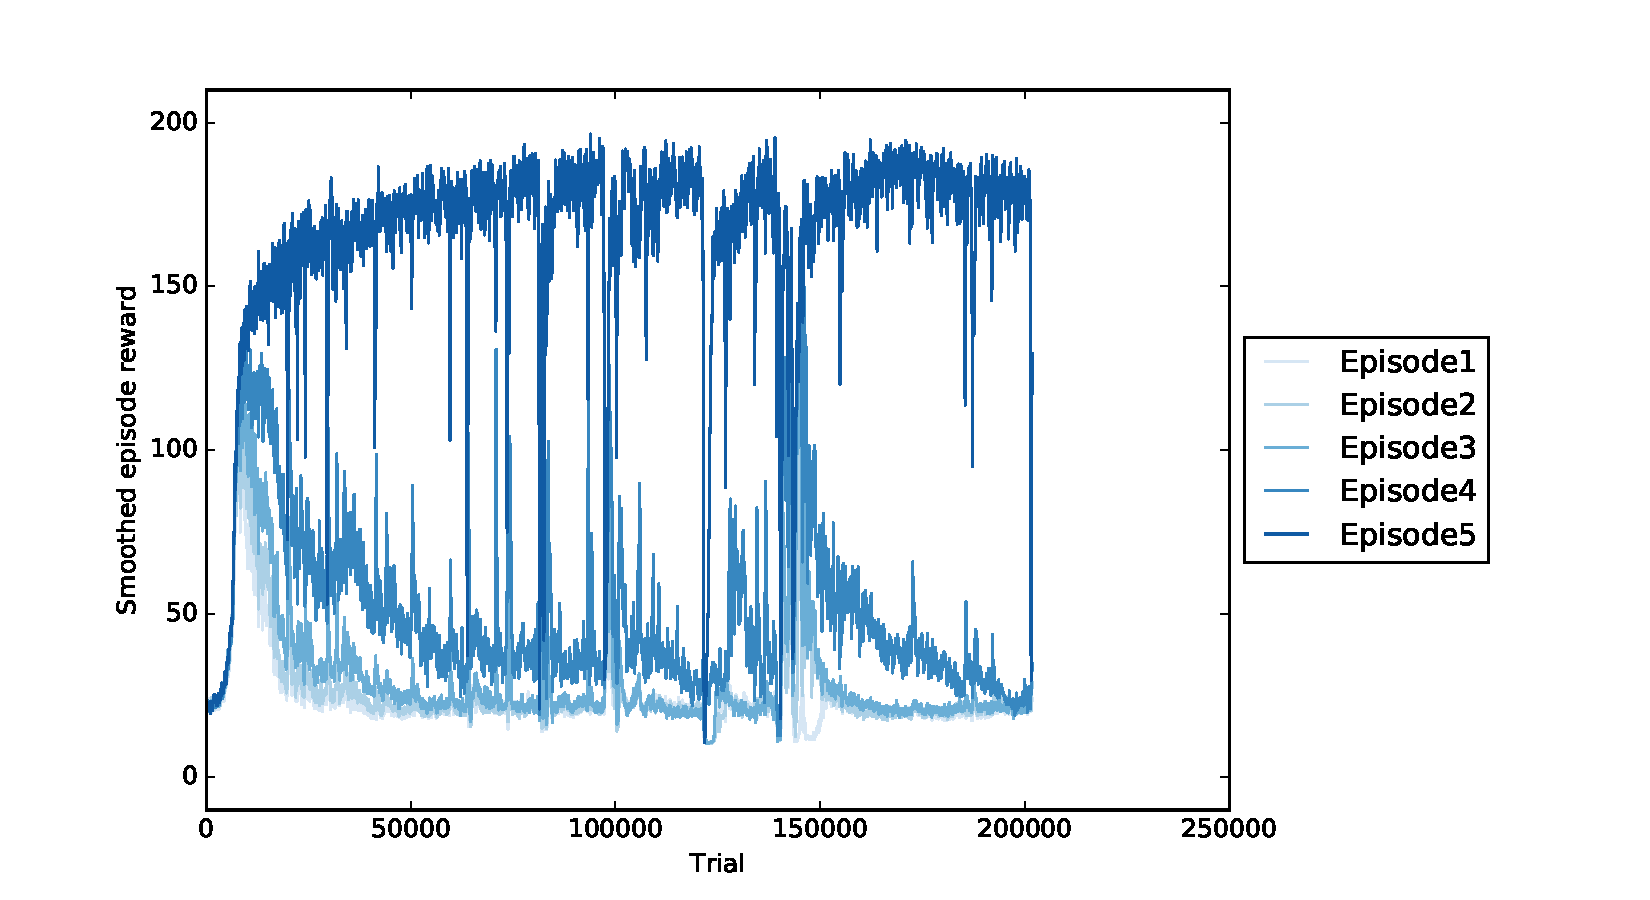
\includegraphics[width=0.49\linewidth]{fig/res_perms5ep_88.pdf}}
	\subfloat[][$\gamma=0.91$]{
		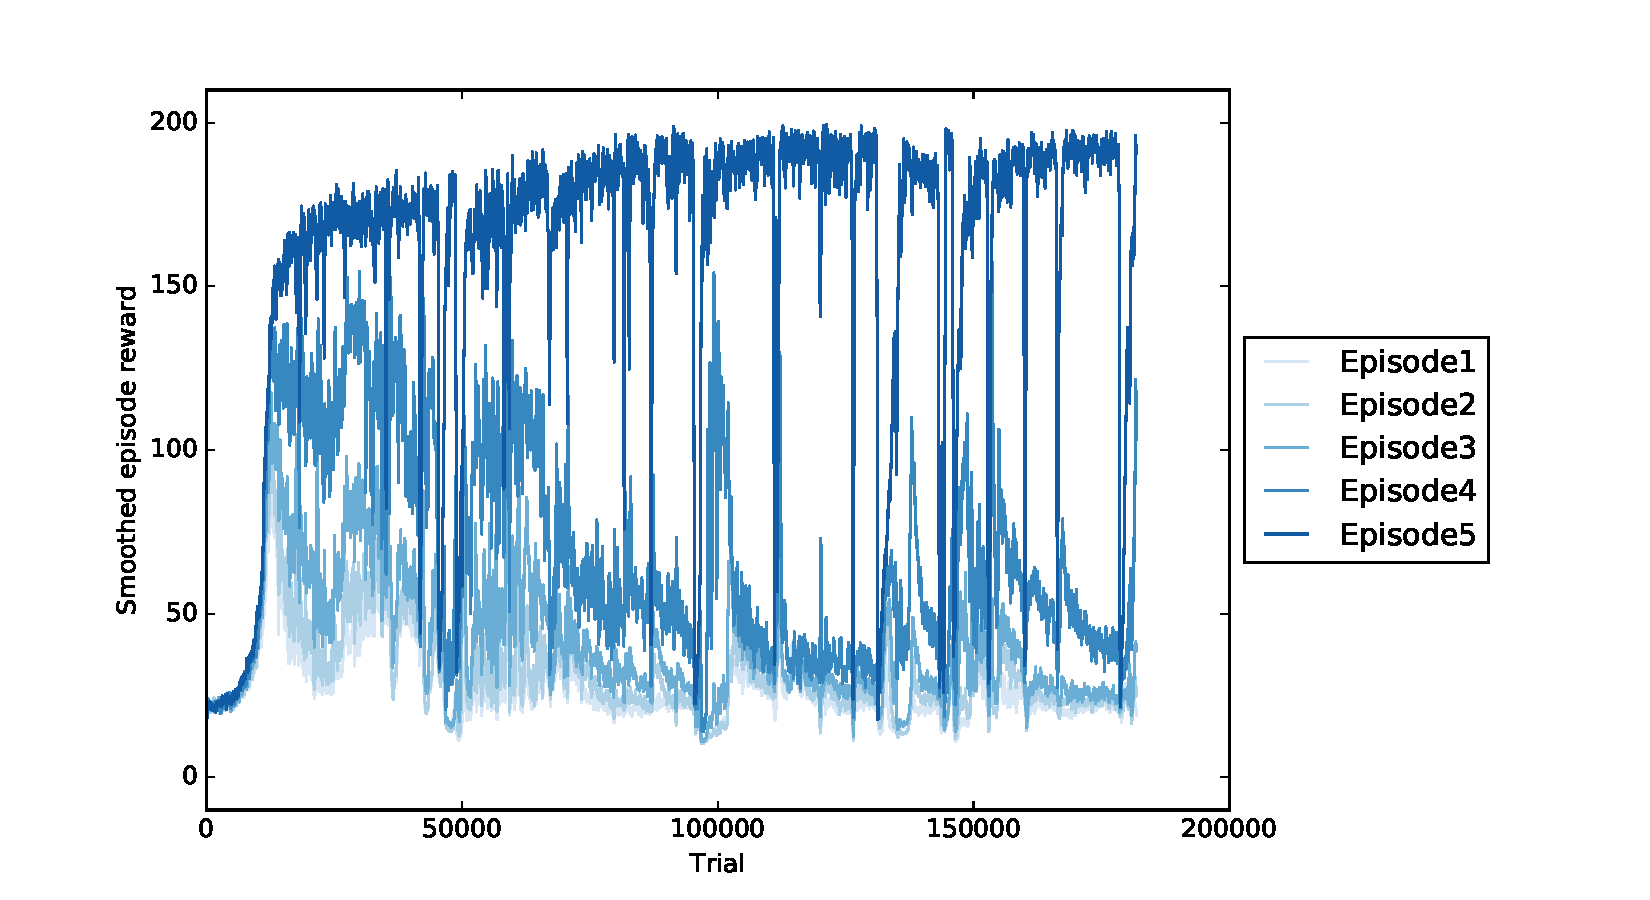
\includegraphics[width=0.49\linewidth]{fig/res_perms5ep_91.pdf}}
	\\
	\subfloat[][$\gamma=0.94$]{
		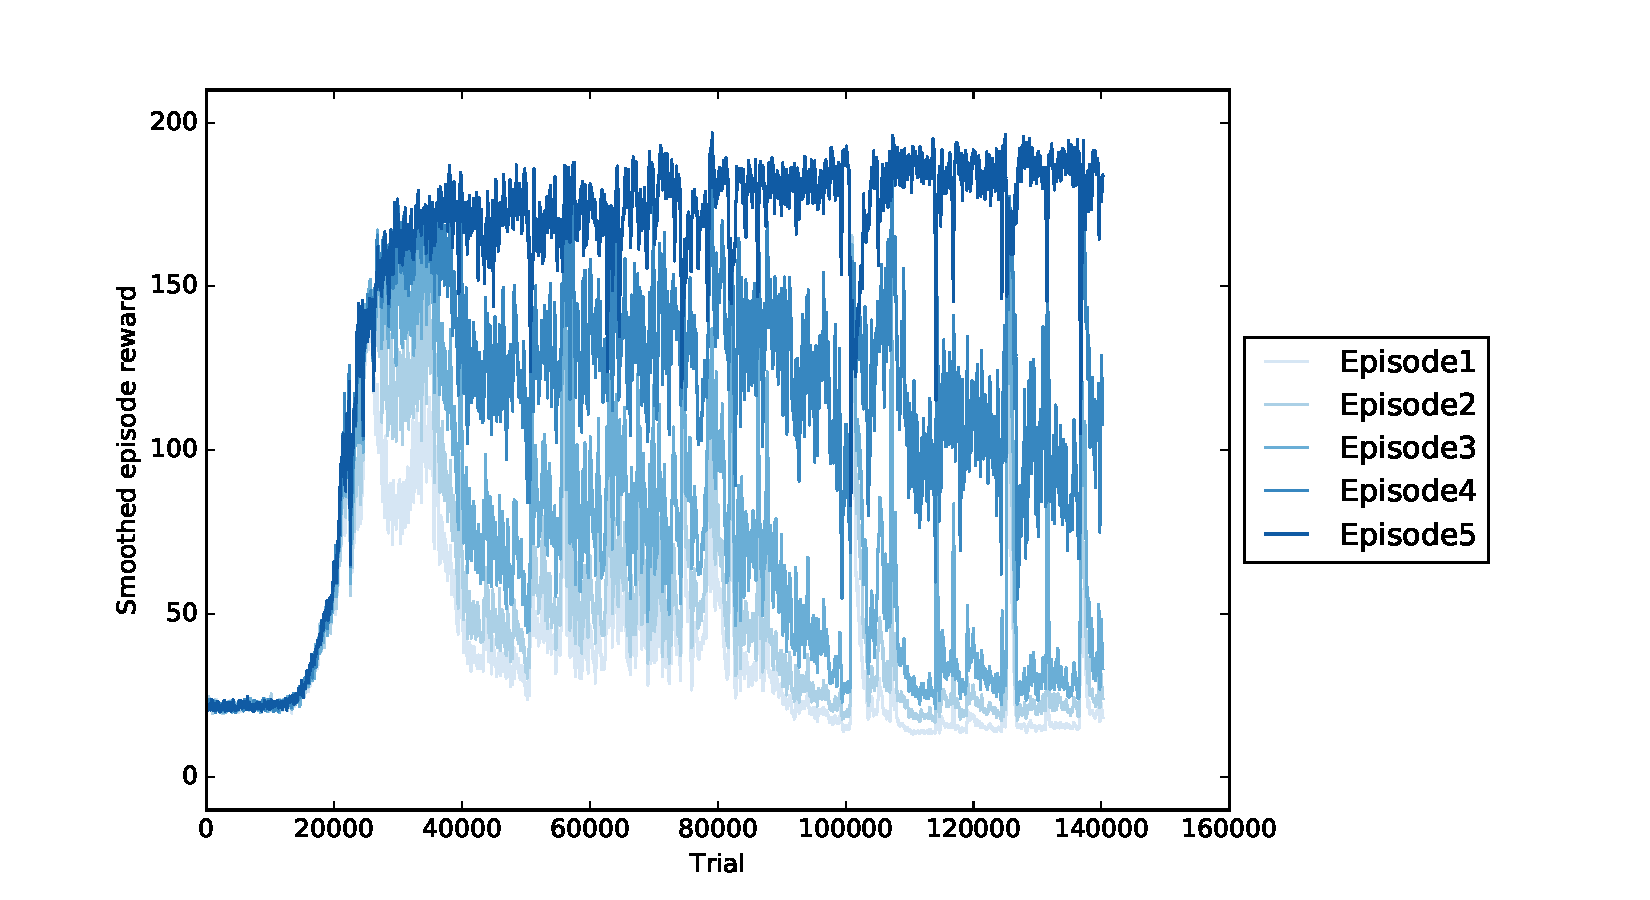
\includegraphics[width=0.49\linewidth]{fig/res_perms5ep_94.pdf}}
	\subfloat[][$\gamma=0.97$]{
		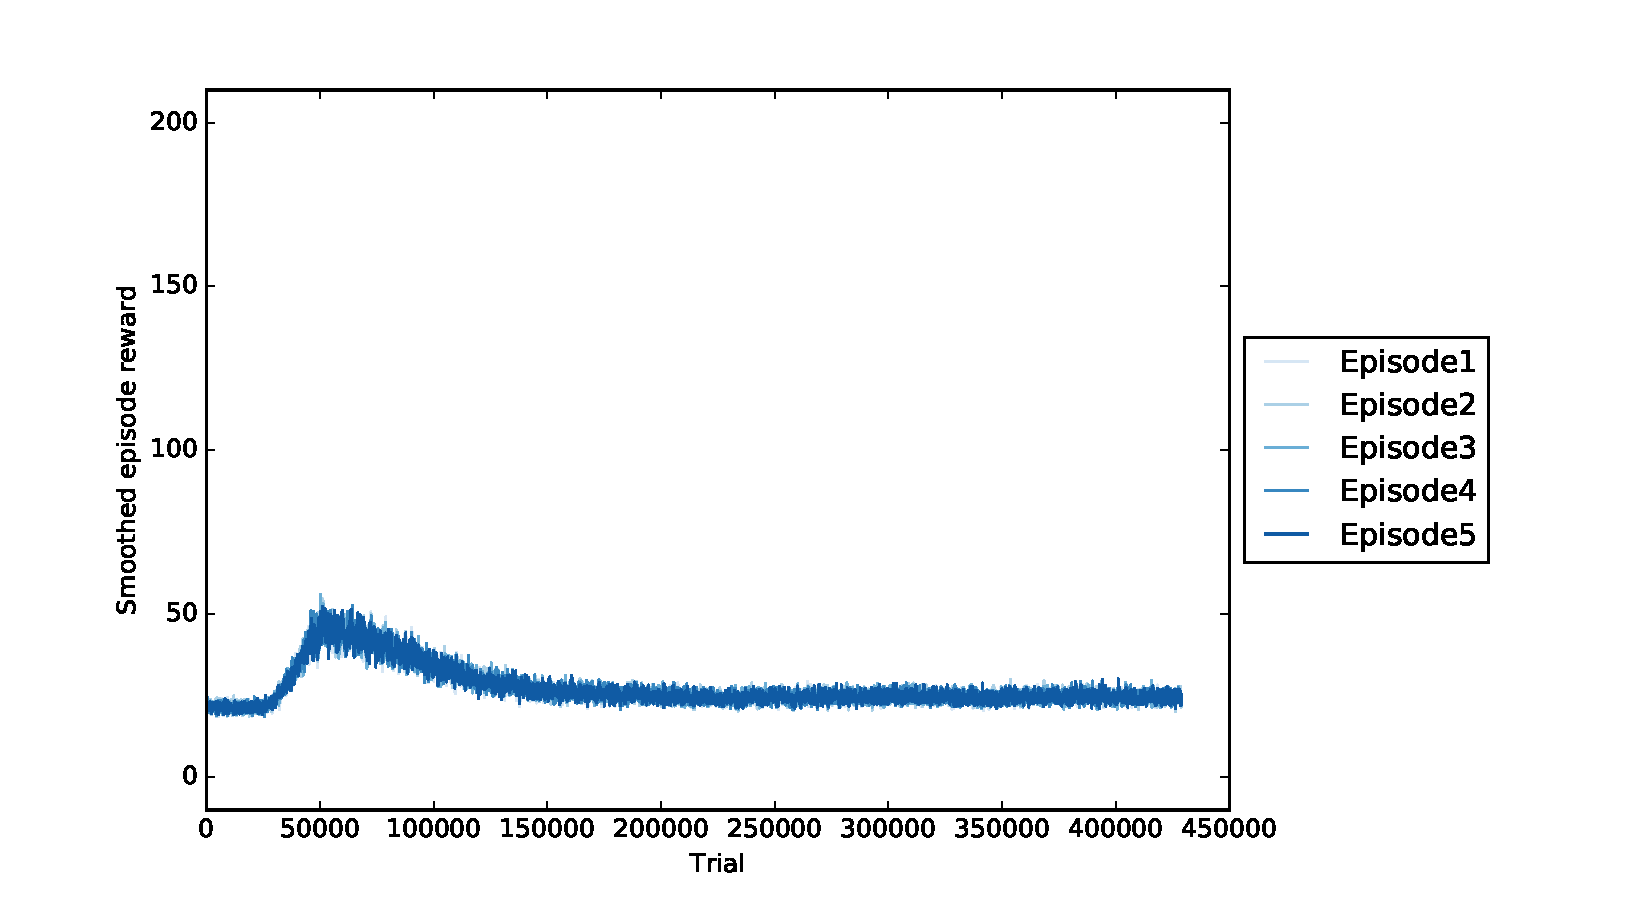
\includegraphics[width=0.49\linewidth]{fig/res_perms5ep_97.pdf}}
	\\
	\caption{Variation of the episode-wise reward evolution in trials of 5
	episodes when tuning the discount factor $\gamma$.}
	\label{fig:varied_gamma}
\end{figure}

\todo{Should I try to explain why and how?}

\subsection{Training on more episodes}
\label{section:beyond:moreeps}
As said before, we made the hypothesis that the agent knew when it was playing
the last episode. What happens if we increase the number of episodes in a
trial? We trained an agent on the permutations shown in table~\ref{tab:3perms}
on trials of 2, 5, 10 and 15 episodes.\\
\begin{figure}
	\centering
	\subfloat[][Trials of 2 episodes]{
		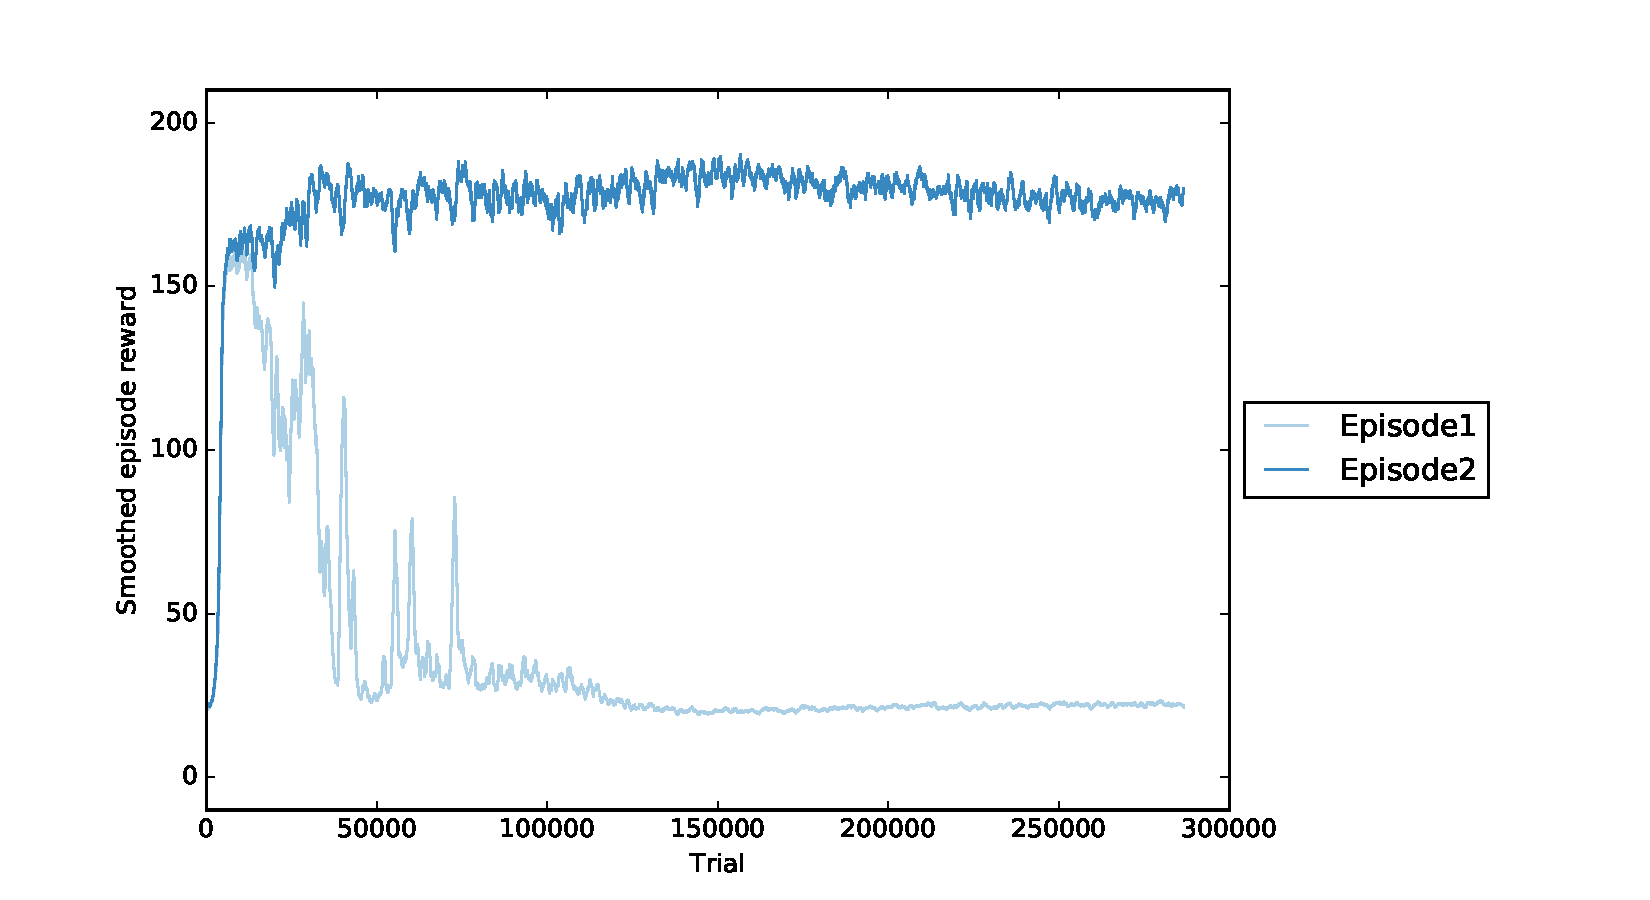
\includegraphics[width=0.49\linewidth]{fig/res_3perms2ep.pdf}}
	\subfloat[][Trials of 5 episodes]{
		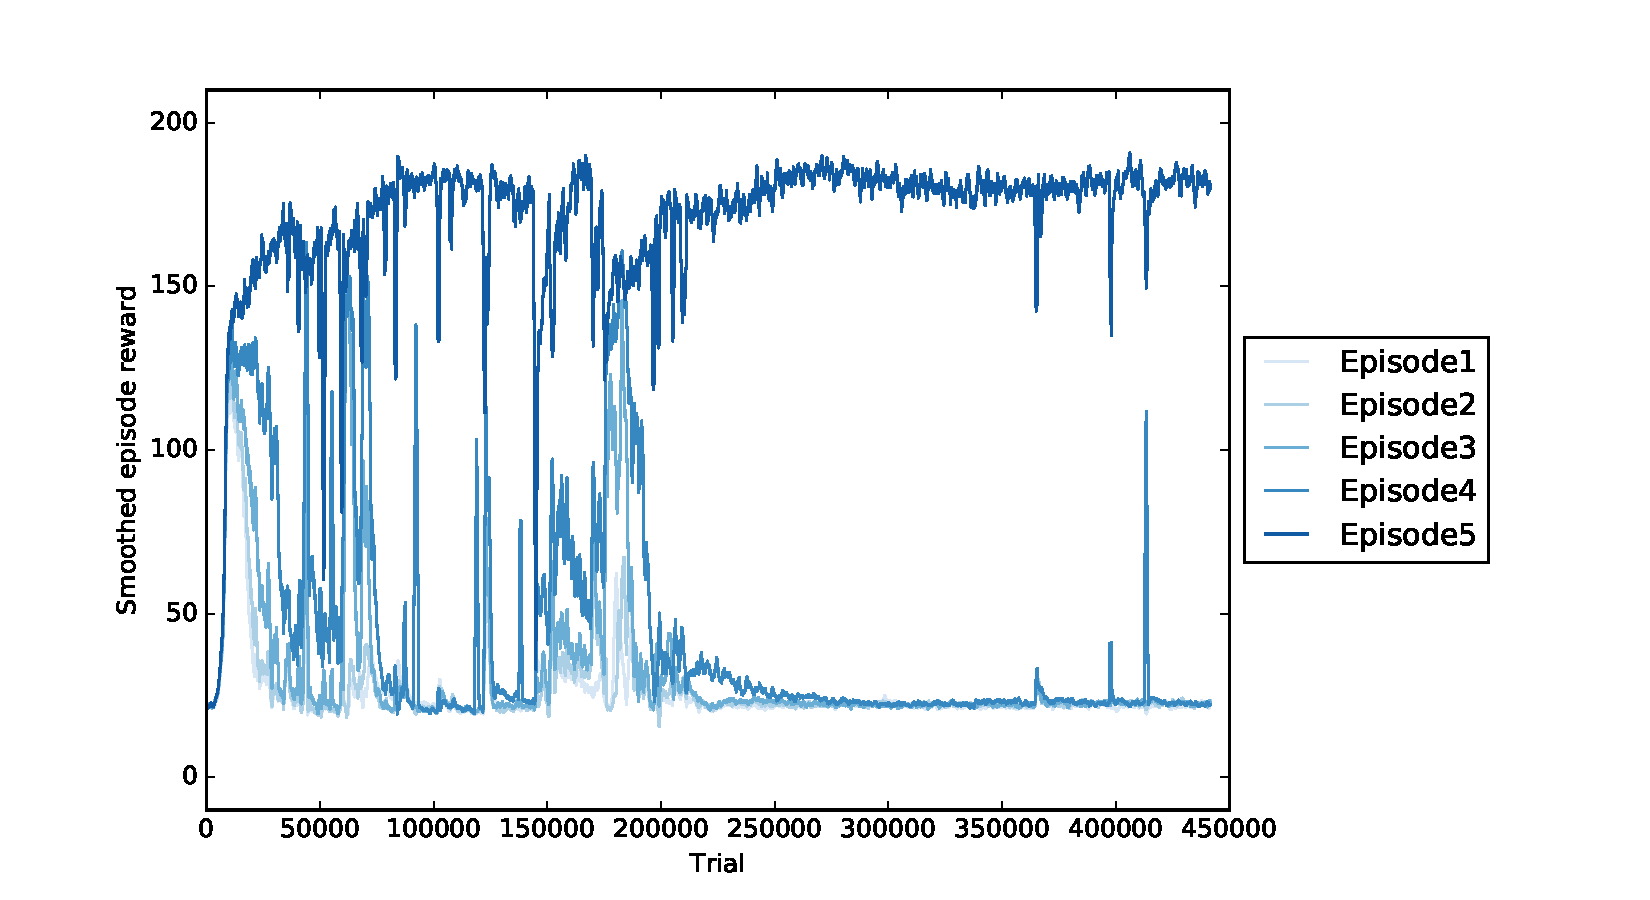
\includegraphics[width=0.49\linewidth]{fig/res_3perms5ep.pdf}}
	\\
	\subfloat[][Trials of 10 episodes]{
		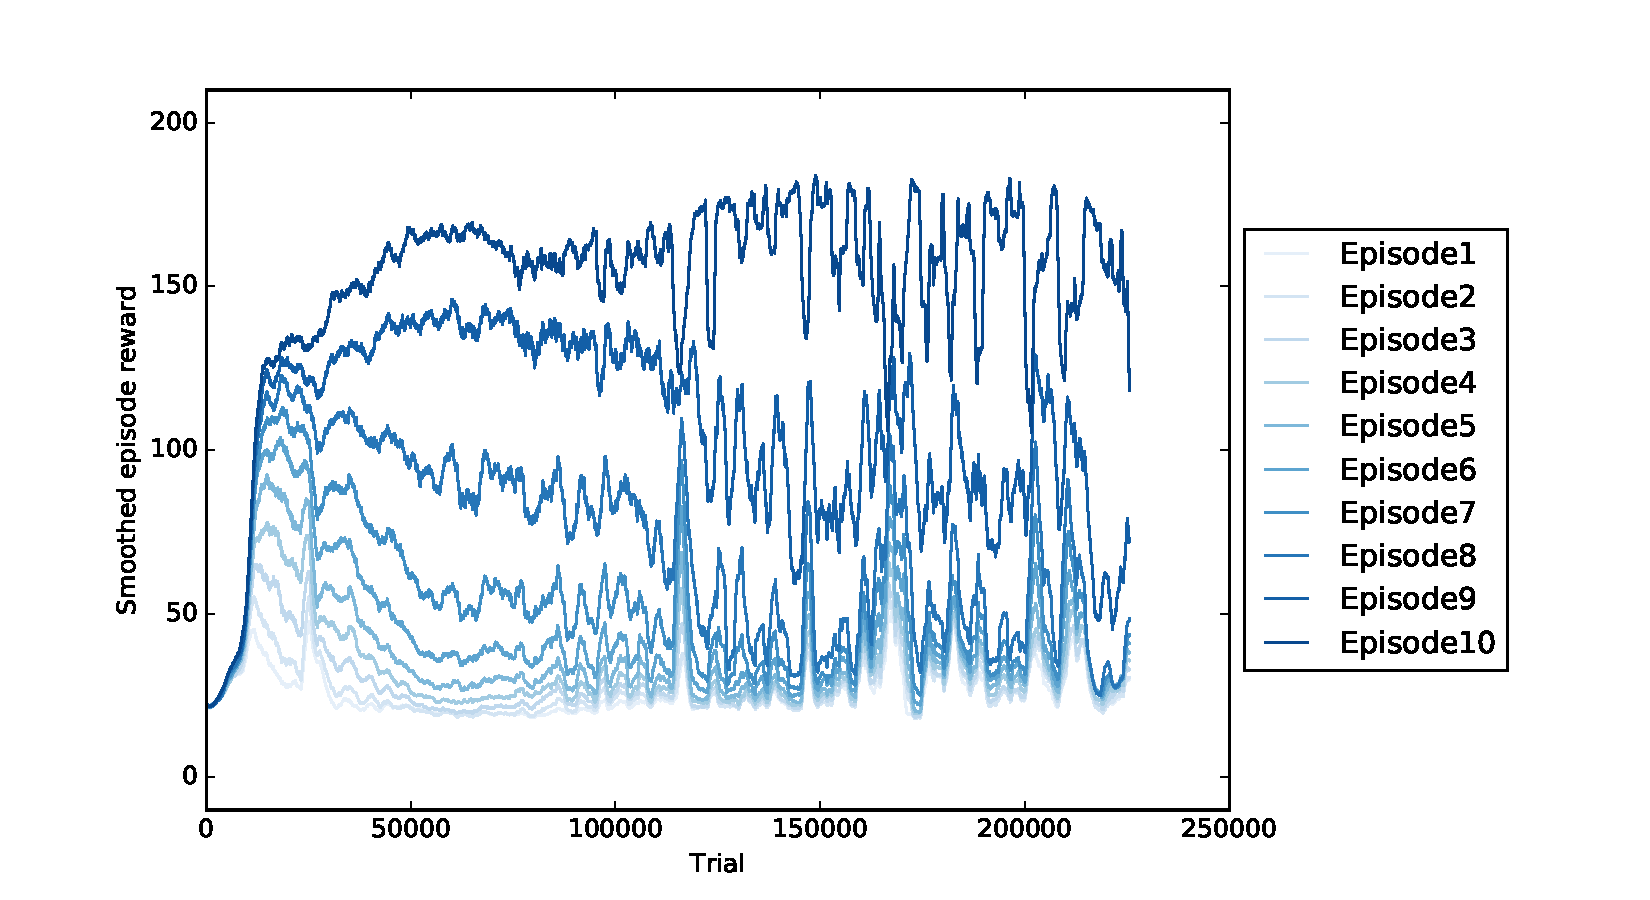
\includegraphics[width=0.49\linewidth]{fig/res_3perms10ep.pdf}}
	\subfloat[][Trials of 15 episodes]{
		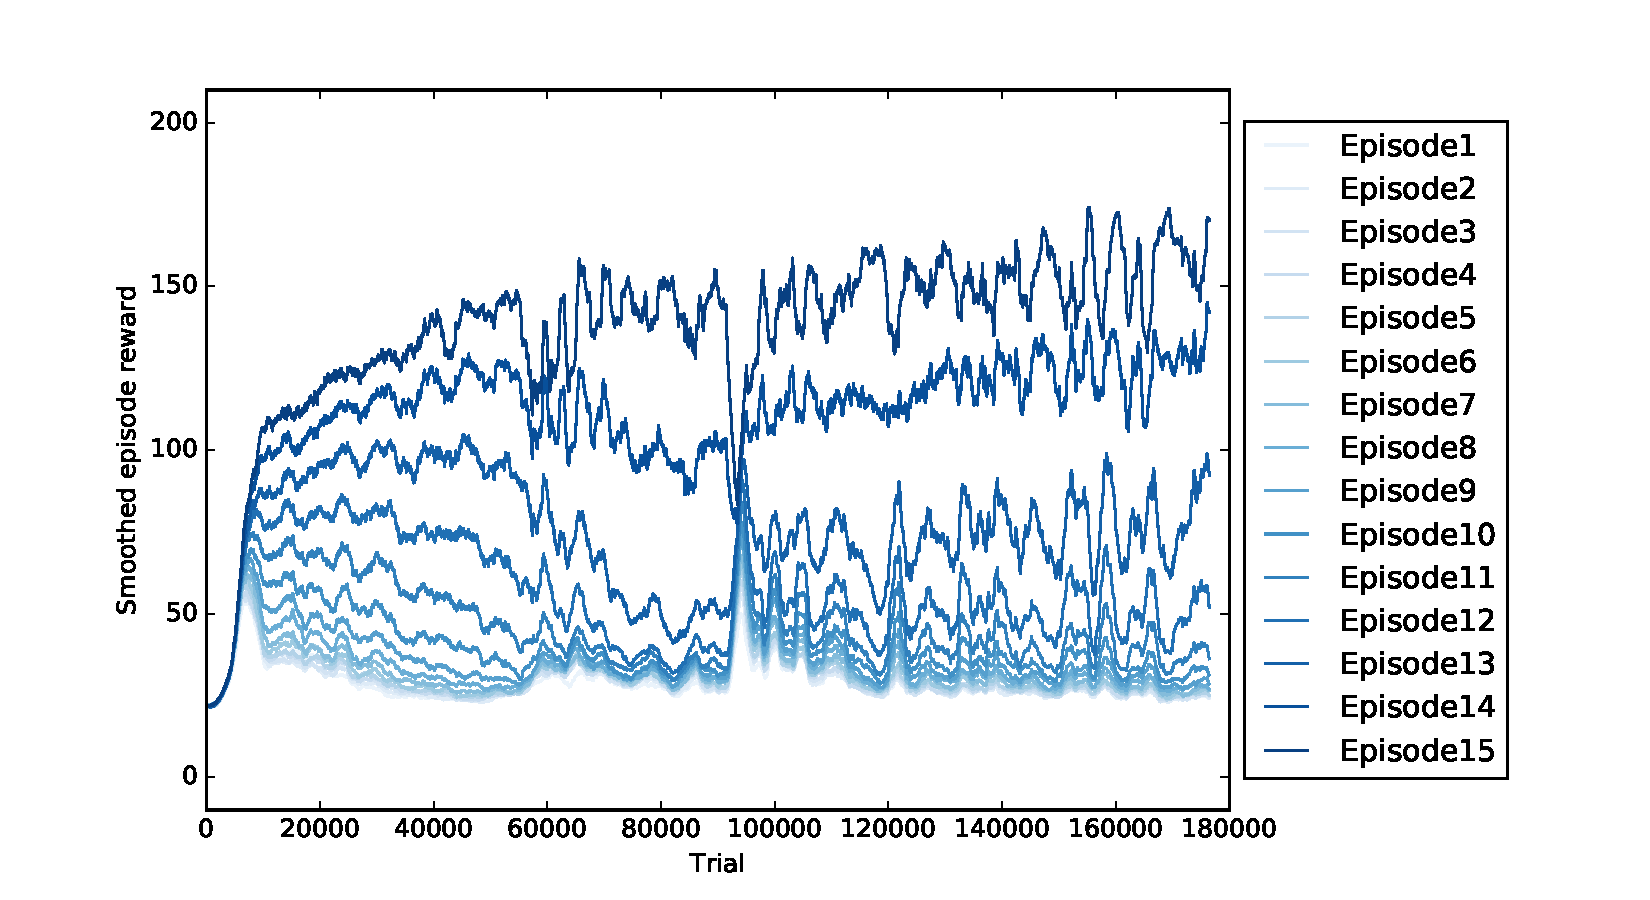
\includegraphics[width=0.49\linewidth]{fig/res_3perms15ep.pdf}}
	\\
	\caption{Episode-wise reward during training with trials of different
	lengths}
	\label{fig:varied_episode_number}
\end{figure}

If we look at the training graphs for this experiment 
(Figure~\ref{fig:varied_episode_number}), we can identify two main trends:
\begin{itemize}
	\item the reward of the last episode doesn't reach optimal performance
		as the number of episodes increases;
	\item the almost last episodes do not fail completely as the number of 
		episodes increases; in fact, in the case of 15 episodes, the
		penultimate episode seems to climb about as much as the last
		episode.
\end{itemize}

From what we can see on Figure~\ref{fig:varied_episode_number}, it looks like
a gain in performance for the last episode always happens at the expense of
the reward of previous episodes. We make the hypothesis that the agent
"counts" the \textbf{timesteps} it takes to reach the last episode. This yields good
performance when the number of timesteps prior to the last episode is stable, 
meaning that all previous episodes have either fail quickly or succeed. Since
the former solution is the simplest to achieve, and it is supported by the 
drop of reward in the first episodes shown on 
Figure~\ref{fig:varied_episode_number}, we believe that is what the agent does.


\section{Testing performance after the training horizon}
So far, we have tested our agent only within the limits of what it has been
trained. What happens if we leave it running for more episodes than what it
has been trained for?


We have trained an agent on the 3 permutations listed in table~\ref{tab:3perms}
without inverted actions, over trials of 5 episodes.
We can test the agent on trials of more episodes - meaning that the hidden
state will be carried on until the end of the 20th episode.
Figure~\ref{fig:horizon_5_3perms} shows the result of this experiment.\\

\begin{figure}
	\centering
	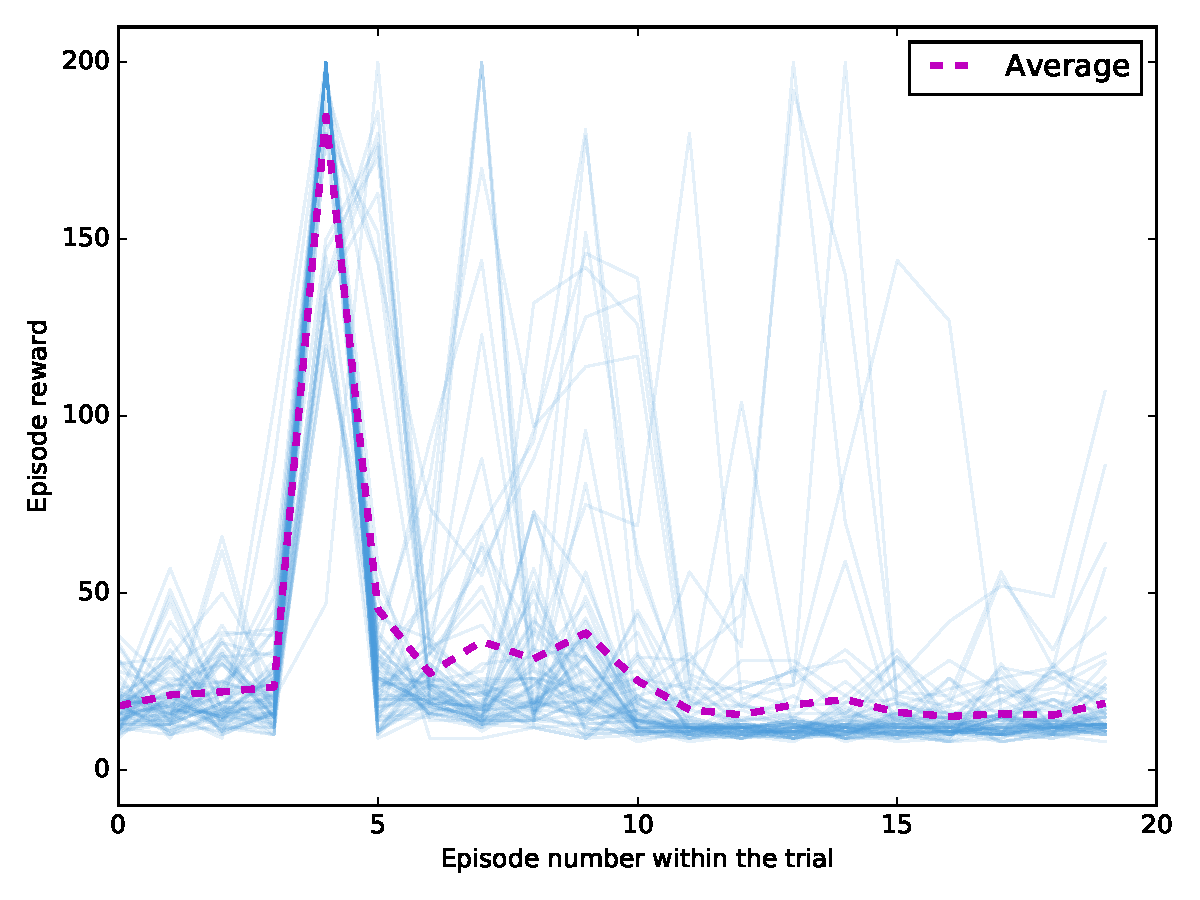
\includegraphics[width=0.8\linewidth]{fig/horizon_5_3perms.pdf}
	\caption{Testing performance over 20 episodes of an agent trained on 
	trials of 5 episodes only. Several runs are shown in blue, their
	average is plotted in red dashes.}
	\label{fig:horizon_5_3perms}
\end{figure}

There is no surprise in the rewards obtained for episodes 0 to 4. The pattern
observed from episode 5 onwards, however, deserves commenting. The first, 
obvious comment to make is that the average reward of the 5th episode is
dramatically low.  There still seems to be mild success after the 5th episode 
until all runs level off to what looks like a random policy level of 
reward.

\subsection{Restoring recurrent weights}
One solution to maintain a high reward after the training horizon would be 
to restore the recurrent weights to their state prior to the last episode of 
the training horizon at the beginning of each episode. As 
Figure~\ref{fig:horizon_5_3perms_restoring} shows, this solution works.\\

\begin{figure}
	\centering
	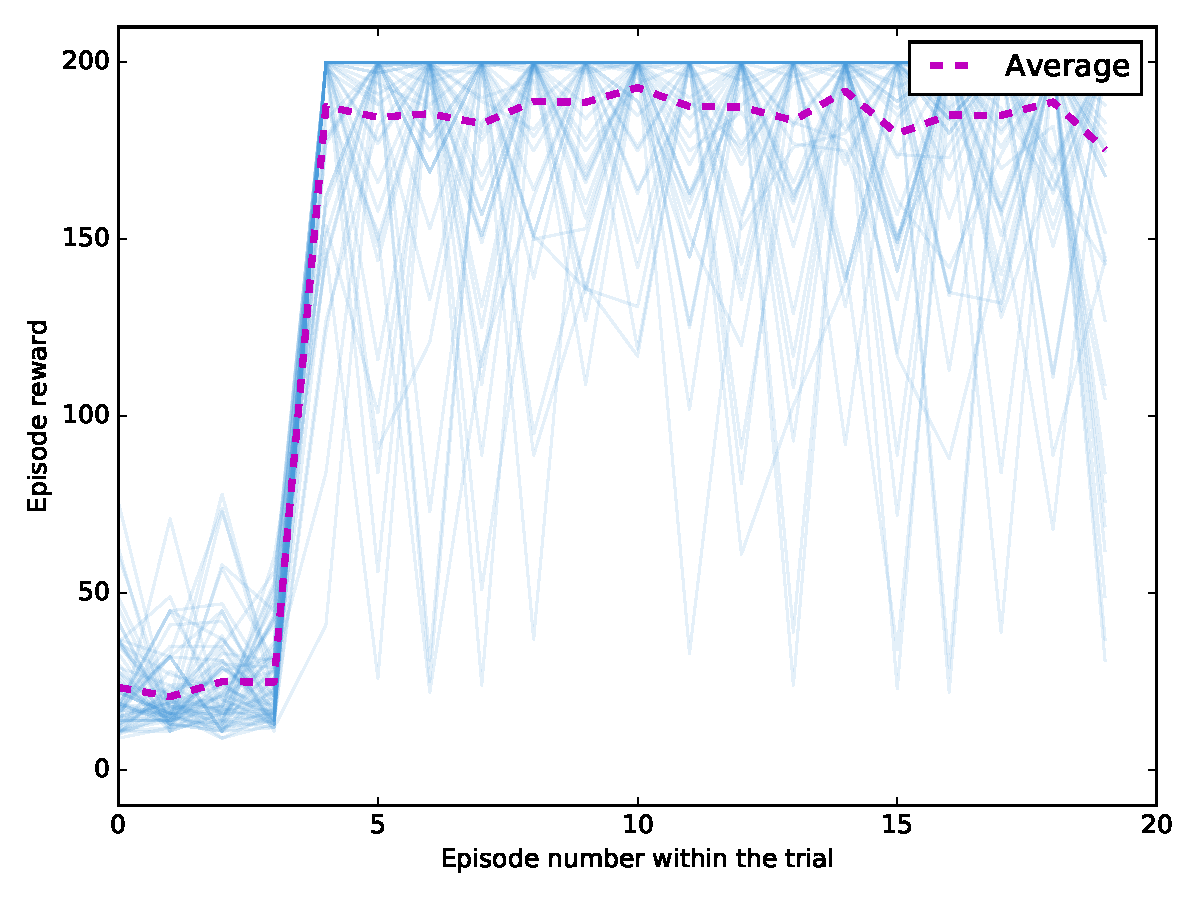
\includegraphics[width=0.8\linewidth]{fig/horizon_5_3perms_restoring.pdf}
	\caption{Testing performance over 20 episodes of an agent trained on 
	trials of 5 episodes only. The recurrent weights are saved prior to 
	the 5th episode and restored prior to each episode from the 6th episode
	onwards. Several runs are shown in blue, their average is plotted in
	red dashes.}
	\label{fig:horizon_5_3perms_restoring}
\end{figure}

This result is not a surprise, and this solution should rather be called a 
workaround. Indeed, restoring the weights at the beginning of each episode
stops any learning to occur after the preset training horizon. Although the
agent is supposed to have reached an optimal policy at the end of the training
horizon, we cannot assume there is nothing left to learn as the agent navigates
through later episodes.\\

Some remarkable feats occur when we we only increase the number of episodes the
agent is trained on. Although it seems the agent doesn't manage to reach
the peak performance of the agent trained on 5 episodes, a few interesting
things to notice are:

\begin{itemize}
	\item the reward in the first 5 to 7 episodes seems to be slightly
		superior to the reward in the first episodes of the agent trained
		on 5 episodes
	\item some of the 9th episodes are successful - and unlike anything
		we have seen so far, they are the penultimate episode -- not
		the last one.
	\item most importantly, the average reward beyond the horizon is
		significantly higher than what we have seen for the agent
		trained on 5 episodes.
\end{itemize}

These findings seem to support the hypothesis we made earlier that the agent
tries to figure out whether or not it is playing the last episode. Pushing
the horizon further seems to confuse the agent's count, forcing it 
to distribute its high performance on several of the last episodes instead
of only the last one.\\

\begin{figure}
	\centering
	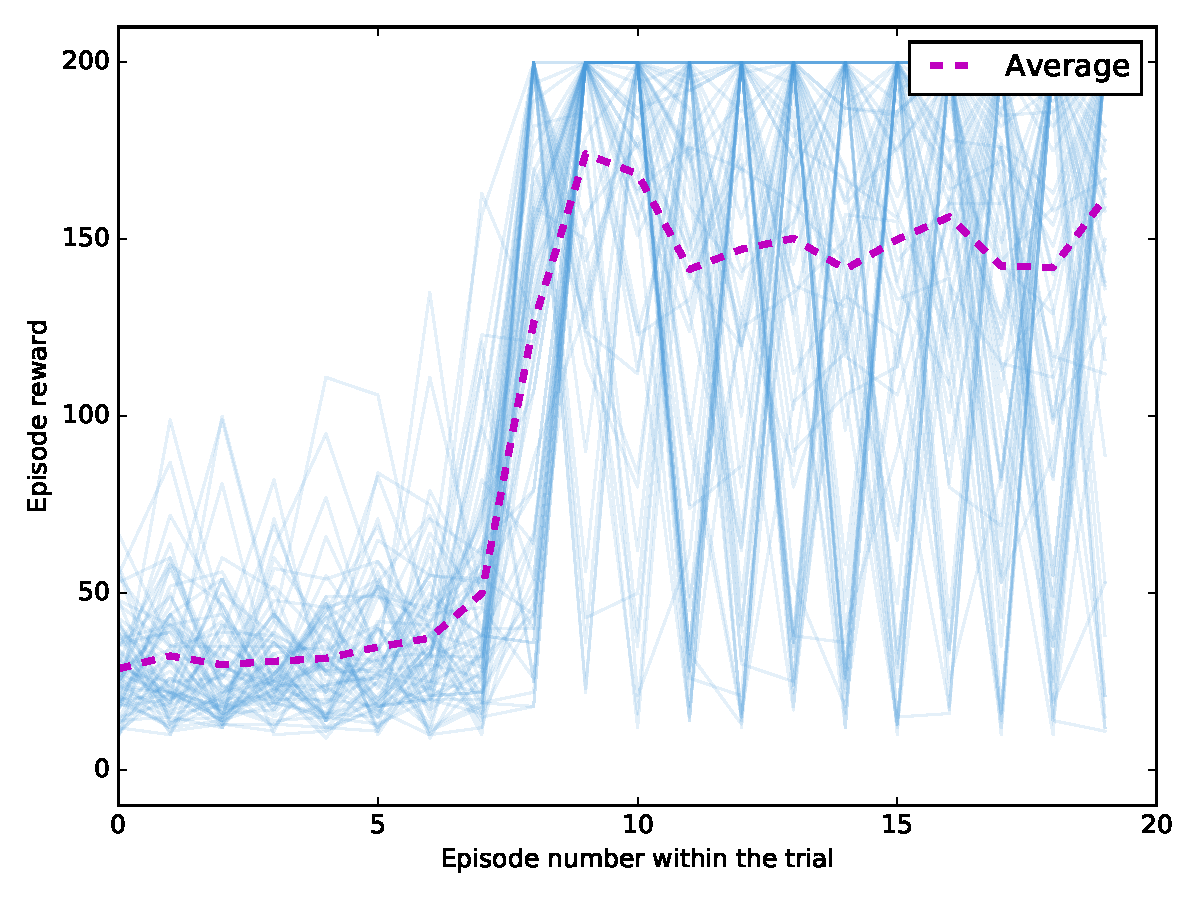
\includegraphics[width=0.8\linewidth]{fig/horizon_10_3perms.pdf}
	\caption{Testing performance over 20 episodes of an agent trained on 
	trials of 10 episodes only. 
	Several runs are shown in blue, their average is plotted in red dashes.}
	\label{fig:horizon_10_3perms}
\end{figure}


